\documentclass[11pt,a4paper]{article}
\usepackage[margin=0.85in]{geometry}
\usepackage{amsmath,amssymb,booktabs,array,xcolor,fancyhdr,hyperref,enumitem,tikz,pgfplots}
\usetikzlibrary{arrows.meta,positioning,calc}
\pgfplotsset{compat=1.18}
\definecolor{navy}{RGB}{25,45,75}
\definecolor{bluegreen}{RGB}{0,125,140}
\definecolor{softgray}{RGB}{95,105,115}
\hypersetup{colorlinks=true,linkcolor=navy}
\pagestyle{fancy}\fancyhf{}\lhead{\small Mathematics Portfolio}\rhead{\small Braess's Paradox}\cfoot{\thepage}
\setlength{\parskip}{7pt}\setlength{\parindent}{0pt}
\newcommand{\sectiontitle}[1]{\section*{\color{navy}#1}}
\newcommand{\network}[2]{%
\begin{tikzpicture}[>=Stealth,thick,every node/.style={circle,draw=navy,fill=navy!8,minimum size=10mm}]
\node (A) at (0,0) {A};\node (B) at (3,1.8) {B};\node (C) at (3,-1.8) {C};\node (D) at (6,0) {D};
\draw[->] (A)--node[above left,draw=none,fill=white] {$x/#1$}(B);
\draw[->] (B)--node[above right,draw=none,fill=white] {$45$}(D);
\draw[->] (A)--node[below left,draw=none,fill=white] {$45$}(C);
\draw[->] (C)--node[below right,draw=none,fill=white] {$x/#1$}(D);
\ifnum#2=1\draw[->,red!75!black,very thick] (B)--node[right,draw=none,fill=white] {$0$}(C);\fi
\end{tikzpicture}}
\begin{document}
\begin{titlepage}
\centering
\vspace*{0.55cm}
{\large\color{bluegreen}\bfseries AN INDEPENDENT MATHEMATICS PROJECT\par}
\vspace{0.65cm}
{\Huge\bfseries Can Adding a Road\\[8pt] Make Traffic Worse?\par}
\vspace{0.35cm}
{\Large\color{navy} Exploring Braess's Paradox Through Mathematical Modeling\par}
\vspace{0.75cm}
\network{100}{1}
\par\vspace{0.55cm}
{\Large\bfseries Asim Nepal\par}
\vspace{0.12cm}
{\large SUNY Brockport\par}
\vspace{0.12cm}
{\normalsize November 2026\par}
\vspace{0.65cm}
\begin{minipage}{0.83\textwidth}
\centering\color{softgray}\itshape
I wanted to bring together the ideas I have learned in my mathematics courses and use them to understand one real question. This project uses traffic networks to show how different parts of mathematics can work together, and why a choice that helps one person may not help everyone.
\end{minipage}
\vfill
{\small\color{softgray}Independent Mathematics Portfolio\par}
\end{titlepage}

\sectiontitle{1. The Question}
Imagine a city with 4,000 drivers. Everyone wants to go from A to D. The city adds a road to help traffic. Will the trip get faster? Not always. In some networks, the new road makes the trip longer. This is called \textbf{Braess's paradox}.

I grew up in Nepal and later moved to the United States for college. I have seen different roads and traffic in both places. That made me curious about how roads work together. In this project, I use math to test what happens when a new road is added.

\textbf{Important:} The Nepal-inspired and U.S.-inspired models below use made-up numbers. They do not measure real traffic in either country. The only difference we test is how quickly a road slows down as more drivers use it.

\sectiontitle{2. Draw the Road Network}
There are four places, $V=\{A,B,C,D\}$. Before adding a road, drivers can take $A\to B\to D$ or $A\to C\to D$.
\begin{center}\network{100}{0}\end{center}
The roads labeled $45$ always take 45 minutes. A road labeled $x/100$ takes $x/100$ minutes when $x$ drivers use it. For example, 2,000 drivers take $2000/100=20$ minutes on that road.

\sectiontitle{3. Calculus I: Why Traffic Gets Slower}
For a road with time $t(x)=x/100$,
\[t'(x)=\frac1{100}>0.\]
So more drivers mean a longer trip. The time spent by all $x$ drivers is
\[C(x)=xt(x)=\frac{x^2}{100}.\]
Then
\[C'(x)=\frac{x}{50},\qquad C''(x)=\frac1{50}>0.\]
The positive second derivative shows that the total cost grows faster as more drivers arrive.

\sectiontitle{4. Before the New Road}
Let $x$ drivers take the upper route. The other $4000-x$ take the lower route. Their travel times are
\[T_U=\frac{x}{100}+45,\qquad T_L=45+\frac{4000-x}{100}.\]
When both routes are used at equilibrium, neither route can be faster than the other:
\[\frac{x}{100}+45=45+\frac{4000-x}{100}.\]
So $x=2000$. Each route takes
\[\boxed{T_{\rm before}=20+45=65\text{ minutes}.}\]

\sectiontitle{5. Add the New Road}
Now we add a road from B to C. In this simple model, the new road takes zero minutes.
\begin{center}\network{100}{1}\end{center}
There are now three routes:
\[P_1: A\to B\to D,\qquad P_2:A\to C\to D,\qquad P_3:A\to B\to C\to D.\]
Suppose all 4,000 drivers take $P_3$. Then $P_3$ takes $40+0+40=80$ minutes. Switching to $P_1$ or $P_2$ would take $40+45=85$ minutes. No one can save time by switching, so this is an equilibrium.
\[\boxed{T_{\rm after}=80\text{ minutes}.}\]
The new road made the trip $80-65=15$ minutes longer, an increase of about $23.08\%$.

\sectiontitle{6. Discrete Math and Linear Algebra}
List the roads in this order: $AB,BD,AC,CD,BC$. The route-road matrix is
\[R=\begin{pmatrix}1&0&1\\1&0&0\\0&1&0\\0&1&1\\0&0&1\end{pmatrix}.\]
Each column is a route. Each row is a road. A 1 means the route uses that road. If $\mathbf p=(p_1,p_2,p_3)^T$ gives the drivers on the three routes, then
\[\mathbf f=R\mathbf p=\begin{pmatrix}p_1+p_3\\p_1\\p_2\\p_2+p_3\\p_3\end{pmatrix}.\]
This tells us the number of drivers on each road. We also need $p_1+p_2+p_3=4000$ and $p_i\geq0$.

\sectiontitle{7. Calculus II: Adding Up Road Costs}
For the congested road, the area under its time curve is
\[F(x)=\int_0^x\frac{s}{100}\,ds=\frac{x^2}{200}.\]
This is not the same as the total driver-minutes $xt(x)$. Adding these integrals for all roads gives a useful function for finding traffic equilibrium when each road's travel time depends only on its own traffic.

\sectiontitle{8. Calculus III: Find the Best Traffic Split}
Now measure drivers in thousands. Let $a,b,c$ be the drivers on routes $P_1,P_2,P_3$, so $a+b+c=4$. The total cost, in thousands of driver-minutes, is
\[C=10(a+c)^2+10(b+c)^2+45a+45b.\]
Using $c=4-a-b$ gives
\[C(a,b)=10(4-b)^2+10(4-a)^2+45(a+b).\]
We must have $a\geq0$, $b\geq0$, and $a+b\leq4$. Take partial derivatives:
\[C_a=20a-35,\qquad C_b=20b-35.\]
Setting them to zero gives $a=b=1.75$, so $c=0.5$. The Hessian is
\[H=\begin{pmatrix}20&0\\0&20\end{pmatrix}.\]
Both eigenvalues are positive, so this feasible point gives the global minimum.
\[C_{\min}=10(2.25)^2+10(2.25)^2+45(3.5)=258.75.\]
The best average travel time is
\[\boxed{258.75/4=64.6875\text{ minutes}.}\]
This is less than the 80 minutes drivers get when each chooses the fastest route for themselves.

\sectiontitle{9. A 3D View of the Original Model}
The surface below shows average travel time. The horizontal axes are the upper-route and lower-route flows, in thousands. The third route gets $c=4-a-b$. Only the triangle $a\geq0$, $b\geq0$, $a+b\leq4$ is allowed.
\begin{center}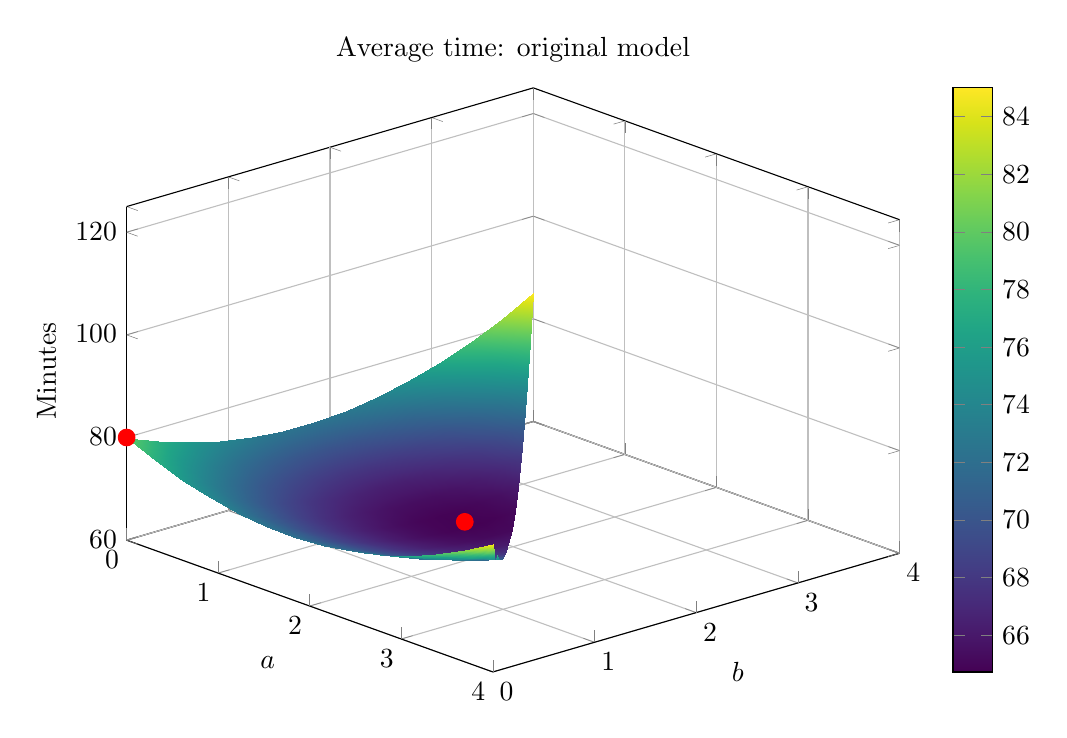
\begin{tikzpicture}\begin{axis}[width=.94\textwidth,height=9cm,view={48}{28},xlabel={$a$},ylabel={$b$},zlabel={Minutes},title={Average time: original model},colormap/viridis,colorbar,grid=major,samples=14,samples y=14,domain=0:4,y domain=0:1,zmin=60,zmax=125]
\addplot3[surf,shader=interp] ({x},{(4-x)*y},{(10*(4-(4-x)*y)^2+10*(4-x)^2+45*(x+(4-x)*y))/4});
\addplot3[only marks,mark=*,mark size=3pt,red] coordinates {(1.75,1.75,64.6875) (0,0,80)};
\end{axis}\end{tikzpicture}\end{center}
The two red points show the best split and the equilibrium after the new road. They are not the same.

\sectiontitle{10. Two Models Inspired by My Experience}
I have seen traffic in Nepal and the United States. I wanted to see how changing one part of the road model changes the result. To keep the comparison fair, both models have the same four places, the same three routes, and 4,000 drivers. Only the crowded roads change.

\begin{center}\begin{tabular}{p{5cm}cc}\toprule
 & Nepal-inspired & U.S.-inspired\\\midrule
Drivers & 4,000 & 4,000\\
Crowded road time & $x/80$ & $x/160$\\
Other road time & 45 min & 45 min\\
New road time & 0 min & 0 min\\\bottomrule
\end{tabular}\end{center}
The Nepal-inspired model gets crowded faster because its travel-time formula has a smaller denominator. This is an assumption for our math experiment, not a claim about real roads.

\subsection*{Nepal-inspired road network}
\begin{center}\network{80}{1}\end{center}
\subsection*{U.S.-inspired road network}
\begin{center}\network{160}{1}\end{center}

\sectiontitle{11. Nepal-Inspired Model: Solve the Math}
\textbf{Before the new road.} Traffic splits equally, with 2,000 drivers on each route:
\[T_{\rm before}=45+\frac{2000}{80}=\boxed{70\text{ minutes}.}\]
\textbf{After the new road.} Let $a$ thousand drivers take each outer route, and $4-2a$ thousand take the middle route. The two crowded roads each carry $4-a$ thousand drivers.

The outer route takes
\[T_{\rm outer}=45+12.5(4-a)=95-12.5a.\]
The middle route takes
\[T_{\rm middle}=25(4-a)=100-25a.\]
At equilibrium, both kinds of route are used, so
\[95-12.5a=100-25a\quad\Longrightarrow\quad \boxed{a=0.4}.\]
That means 400 drivers use each outer route and 3,200 drivers use the middle route. Every used route takes
\[\boxed{T_{\rm after}=90\text{ minutes}.}\]
The new road adds $90-70=\boxed{20}$ minutes to the average trip.

\sectiontitle{12. U.S.-Inspired Model: Solve the Math}
\textbf{Before the new road.} Again, 2,000 drivers take each route:
\[T_{\rm before}=45+\frac{2000}{160}=\boxed{57.5\text{ minutes}.}\]
\textbf{After the new road.} Suppose everyone uses the middle route. Its time is
\[T_{\rm middle}=\frac{4000}{160}+\frac{4000}{160}=\boxed{50\text{ minutes}.}\]
Either outer route would take $25+45=70$ minutes. So no driver wants to switch. All 4,000 drivers using the middle route is an equilibrium.

The new road saves $57.5-50=\boxed{7.5}$ minutes per driver.

\sectiontitle{13. Compare Both Models}
\begin{center}\renewcommand{\arraystretch}{1.4}\begin{tabular}{p{5.2cm}cc}\toprule
 & Nepal-inspired & U.S.-inspired\\\midrule
Before the road & 70 min & 57.5 min\\
After the road & 90 min & 50 min\\
Change & $+20$ min & $-7.5$ min\\
Result & Worse & Better\\\bottomrule
\end{tabular}\end{center}
\begin{center}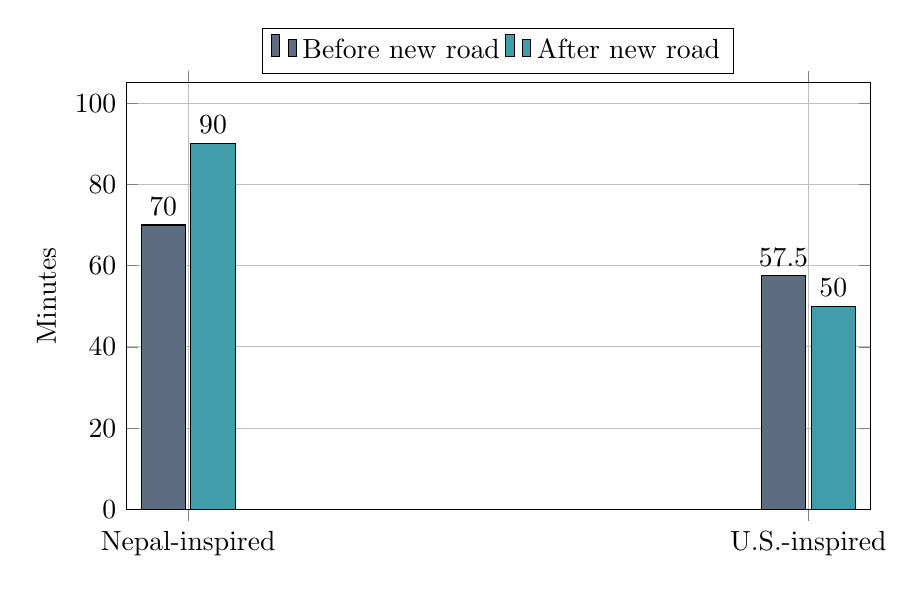
\begin{tikzpicture}\begin{axis}[ybar,bar width=16pt,width=.91\textwidth,height=7cm,ymin=0,ymax=105,ylabel={Minutes},symbolic x coords={Nepal-inspired,U.S.-inspired},xtick=data,legend style={at={(.5,1.02)},anchor=south,legend columns=2},nodes near coords,grid=major]
\addplot[fill=navy!70] coordinates {(Nepal-inspired,70) (U.S.-inspired,57.5)};
\addplot[fill=bluegreen!75] coordinates {(Nepal-inspired,90) (U.S.-inspired,50)};
\legend{Before new road,After new road}
\end{axis}\end{tikzpicture}\end{center}
The same road change gives different results because the crowded roads have different cost functions. That is why the whole network matters.

\sectiontitle{14. Calculus III: Best Split in Each Model}
Let $k$ be the number in the crowded-road formula $t(x)=x/k$. With traffic measured in thousands, the total cost is
\[C_k(a,b)=\frac{1000}{k}\big[(4-a)^2+(4-b)^2\big]+45(a+b).\]
Here $a,b\geq0$ and $a+b\leq4$. The partial derivatives are
\[\frac{\partial C_k}{\partial a}=\frac{2000}{k}(a-4)+45,\qquad
\frac{\partial C_k}{\partial b}=\frac{2000}{k}(b-4)+45.\]
The unconstrained critical point is
\[a=b=4-\frac{45k}{2000}.\]
\textbf{Nepal-inspired model ($k=80$).} The critical point is $a=b=2.2$, but $a+b=4.4>4$. It is not allowed. The minimum lies on the boundary $a+b=4$. On that boundary, symmetry and the convex cost give $a=b=2$, $c=0$. The average is
\[\boxed{T_{\rm best,N}=70\text{ minutes}.}\]
\textbf{U.S.-inspired model ($k=160$).} The critical point is $a=b=0.4$, which is allowed. Then $c=3.2$. Its total cost is
\[C=6.25(3.6)^2+6.25(3.6)^2+45(0.8)=198.\]
So the best average is
\[\boxed{T_{\rm best,U}=198/4=49.5\text{ minutes}.}\]
Both cost functions are convex. Checking the allowed triangle gives these global minimum values.

\sectiontitle{15. Two 3D Cost Surfaces}
Each surface shows the average time for different choices of $a$ and $b$. A lower point means less time.
\begin{center}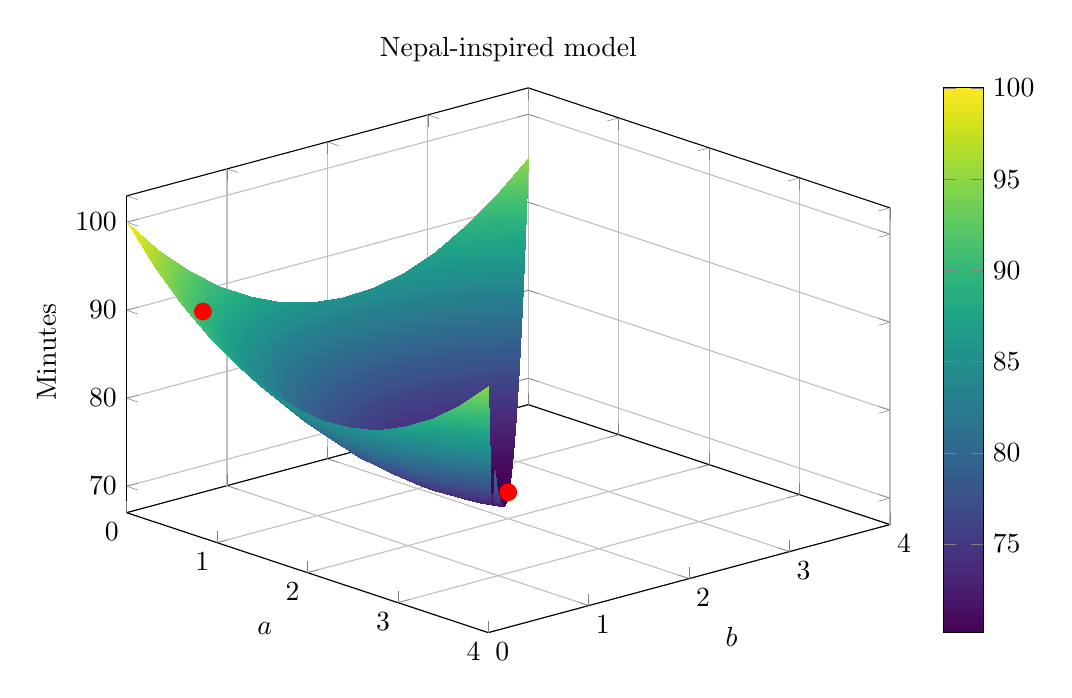
\begin{tikzpicture}\begin{axis}[width=.93\textwidth,height=8.5cm,view={48}{27},xlabel={$a$},ylabel={$b$},zlabel={Minutes},title={Nepal-inspired model},colormap/viridis,colorbar,grid=major,samples=14,samples y=14,domain=0:4,y domain=0:1]
\addplot3[surf,shader=interp] ({x},{(4-x)*y},{(12.5*(4-(4-x)*y)^2+12.5*(4-x)^2+45*(x+(4-x)*y))/4});
\addplot3[only marks,red,mark=*,mark size=3pt] coordinates {(2,2,70) (.4,.4,90)};
\end{axis}\end{tikzpicture}\end{center}
\begin{center}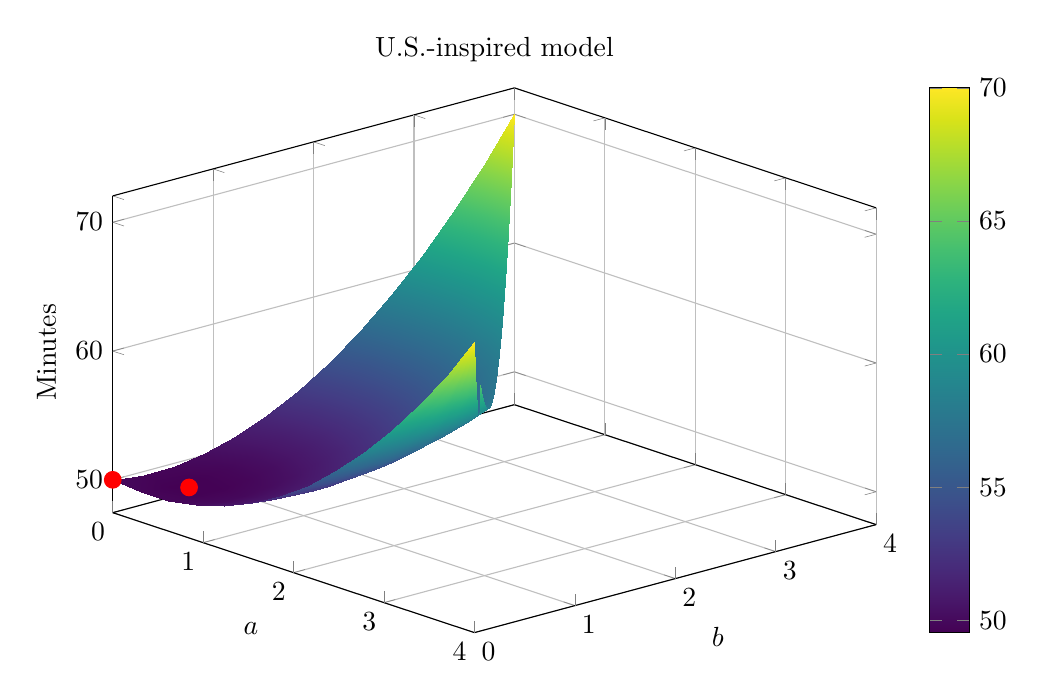
\begin{tikzpicture}\begin{axis}[width=.93\textwidth,height=8.5cm,view={48}{27},xlabel={$a$},ylabel={$b$},zlabel={Minutes},title={U.S.-inspired model},colormap/viridis,colorbar,grid=major,samples=14,samples y=14,domain=0:4,y domain=0:1]
\addplot3[surf,shader=interp] ({x},{(4-x)*y},{(6.25*(4-(4-x)*y)^2+6.25*(4-x)^2+45*(x+(4-x)*y))/4});
\addplot3[only marks,red,mark=*,mark size=3pt] coordinates {(.4,.4,49.5) (0,0,50)};
\end{axis}\end{tikzpicture}\end{center}
The red dots mark the best split and the equilibrium. They show how close or far the drivers' choices are from the lowest possible average time.

\sectiontitle{16. A New Question: When Does the Paradox Happen?}
Instead of choosing only $k=80$ or $k=160$, let $k$ change. This lets us study many possible road conditions.

Before the new road, the average time is
\[T_{\rm before}(k)=45+\frac{2000}{k}.\]
If all drivers use the middle route, it takes $8000/k$ minutes. This is an equilibrium when switching to an outer route cannot save time:
\[\frac{8000}{k}\leq45+\frac{4000}{k}\quad\Longleftrightarrow\quad k\geq\frac{4000}{45}.\]
For smaller $k$, there is an equilibrium where all three routes are used. Let $a$ thousand drivers use each outer route. Setting outer and middle times equal gives
\[45+\frac{1000(4-a)}{k}=\frac{2000(4-a)}{k},\]
so
\[a=4-\frac{45k}{1000}.\]
This value is between 0 and 2 when $4000/90\leq k\leq4000/45$. In this range, the common travel time is $90$ minutes.

For $k<4000/90$, the new middle road is not used at equilibrium; the two old routes still take $45+2000/k$ minutes. Therefore,
\[
T_{\rm after}(k)=
\begin{cases}
45+2000/k, & 0<k\leq 4000/90,\\
90, & 4000/90<k<4000/45,\\
8000/k, & k\geq4000/45.
\end{cases}
\]
Compare this with $T_{\rm before}(k)$. The new road makes traffic strictly worse exactly when
\[\boxed{\frac{4000}{90}<k<\frac{6000}{45}.}\]
That is about $44.44<k<133.33$. Our Nepal-inspired model has $k=80$, inside this range. Our U.S.-inspired model has $k=160$, outside it.

\begin{center}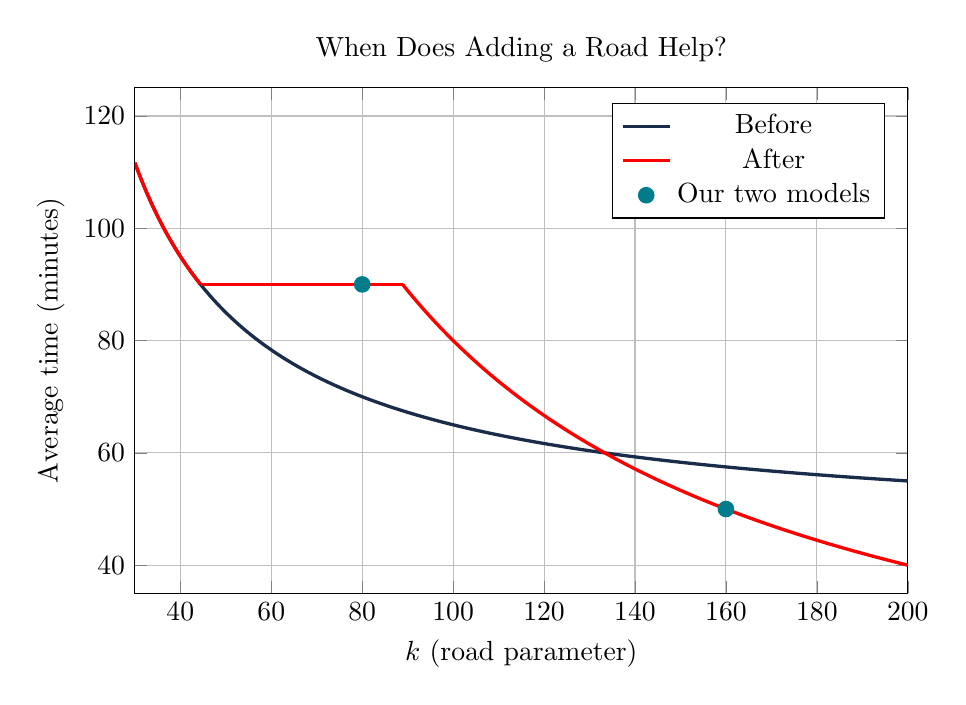
\begin{tikzpicture}\begin{axis}[width=.94\textwidth,height=8cm,xmin=30,xmax=200,ymin=35,ymax=125,xlabel={$k$ (road parameter)},ylabel={Average time (minutes)},title={When Does Adding a Road Help?},grid=both,legend pos=north east]
\addplot[navy,very thick,domain=30:200,samples=200]{45+2000/x};\addlegendentry{Before}
\addplot[red,very thick,domain=30:44.444,samples=50]{45+2000/x};
\addplot[red,very thick,domain=44.444:88.888,samples=50,forget plot]{90};
\addplot[red,very thick,domain=88.888:200,samples=100,forget plot]{8000/x};
\addlegendentry{After}
\addplot[only marks,mark=*,mark size=2.8pt,bluegreen] coordinates {(80,90) (160,50)};\addlegendentry{Our two models}
\end{axis}\end{tikzpicture}\end{center}

\sectiontitle{17. What I Learned}
I started with a simple question about roads. Then I found that adding a road can help, hurt, or make no difference. The answer depends on how the roads work together.

I used graphs to draw the network, matrices to count traffic on each road, derivatives to study changes, integrals to build a traffic function, and partial derivatives to find the best split.

The two models helped me see why changing one number can change the whole result. I also found the exact range of road parameters where the paradox happens. The main lesson is that adding something new does not always make the full system better.

\sectiontitle{18. What I Could Try Next}
\begin{enumerate}[leftmargin=*]
\item Give the new road a travel time greater than zero.
\item Change the total number of drivers.
\item Try different road-time formulas, such as $t(x)=\alpha x^2$.
\item Build a bigger network and use a larger route-road matrix.
\item Use real traffic data, if I can find a reliable dataset, and check how well this simple model works.
\end{enumerate}

\sectiontitle{References}
\begin{enumerate}[leftmargin=*]
\item Braess, D. (1968). \textit{\"Uber ein Paradoxon aus der Verkehrsplanung}. Unternehmensforschung, 12, 258--268.
\item Roughgarden, T. (2005). \textit{Selfish Routing and the Price of Anarchy}. MIT Press.
\end{enumerate}
\end{document}
